%-------------------------------------------------------------------------------
\section{Results}
\label{sec:result}
%-------------------------------------------------------------------------------

This section presents the results obtained from the individual channel, as well as their combination,
following the statistical analysis discussed in Section~\ref{sec:stat_analysis}.

A binned likelihood fit under the signal-plus-background hypothesis is performed on the BDT discriminant distributions in the seven 
analysis regions considered. The unconstrained parameter of the fit are the signal 
strength.
%and four independent parameters associated with the normalisation of the fake $\had$ background in each of the analysis regions. 
No significant pulls or constraints are obtained for the fitted nuisance parameters, resulting in a post-fit background prediction in each analysis region that is
very close to the pre-fit prediction, albeit with reduced uncertainties due to the anti-correlations among sources of systematic uncertainty resulting from the fit.
Figure~\ref{fig:Bonlyfit_data} shows a background only fit to the BDT discriminant distribution in the data.
Figure~\ref{fig:asimov_postfitbdtHc} and~\ref{fig:asimov_postfitbdtHu} show a post-fit with signal plus background (S+B) to the data for
the $tcH$ and $tuH$ search separately.
%both pre- and post-fit to data, in the case of the $\Hc$ search.  
%A similar comparison for the leptonic channel is shown in Figure~\ref{fig:tthML_trexPrefit} and \ref{fig:tthML_trexPrefit_1}.
The observed and predicted yields after fit to the data with background only are summarized in Table~\ref{tab:HtautauPostfitYieldsUnblind}.
%pre-fit and post-fit yields can be found in Appendix~\ref{sec:prepostfit_yields_Htautau_appendix}.
There is an excess of data events above background with a significance of 2.6$\sigma$ in the $t_l\thadhad$ channel in the hight BDT region.
We have checked the kinematic distributions for these excess of events in
the BDT$>0.8$ region and found there are nothing unusual between data and expectation.

\begin{figure}[H]
\centering
\begin{tabular}{@{}ccc@{}}
\includegraphics[width=0.33\textwidth]{\FCNCFigures/unblinded/tthML/tcH_reg1l2tau1bnj_os_postFit_BOnly.pdf}&
\includegraphics[width=0.33\textwidth]{\FCNCFigures/unblinded/tthML/tcH_reg1l1tau1b1j_ss_postFit_BOnly.pdf}&
\includegraphics[width=0.33\textwidth]{\FCNCFigures/unblinded/tthML/tcH_reg1l1tau1b2j_ss_postFit_BOnly.pdf}\\
(a1) BDT dicriminant in $t_l\thadhad$ & (a2) BDT dicriminant in  $t_l\tauhad$-1j& (a3) BDT dicriminant in $t_l\tauhad$-2j\\
\includegraphics[width=0.33\textwidth]{\FCNCFigures/unblinded/tthML/tcH_reg1l1tau1b2j_os_postFit_BOnly.pdf}&
\includegraphics[width=0.33\textwidth]{\FCNCFigures/unblinded/tthML/tcH_reg1l1tau1b3j_os_postFit_BOnly.pdf}&
\includegraphics[width=0.33\textwidth]{\FCNCFigures/unblinded/xTFW/tcH_reg2mtau1b2jos_vetobtagwp70_highmet_postFit_BOnly.pdf}\\
(b1) BDT dicriminant in $t_h\tlhad$-2j & (b2) BDT dicriminant in  $t_h\tlhad$-3j & (b3) BDT dicriminant in $t_h\thadhad$-2j \\
\includegraphics[width=0.33\textwidth]{\FCNCFigures/unblinded/xTFW/tcH_reg2mtau1b3jos_vetobtagwp70_highmet_postFit_BOnly.pdf}& \\
(c1) BDT dicriminant in$t_h\thadhad$-3j\\
\end{tabular}
\caption{ The BDT output distributions are fitted with background only to the data: $t_l\thadhad$ (a1),  $t_l\tauhad$-1j (a2),  $t_l\tauhad$-2j (a3),
  $t_h\tlhad$-2j (b1), $t_h\tlhad$-3j (b2), $t_h\thadhad$-2j (b3), and $t_h\thadhad$-3j (c1).
  Statistical and systematic uncertainties are being shown. The different type of signals are also shown for shape comparision.}
\label{fig:Bonlyfit_data}
\end{figure}


%\input{\FCNCFigures/tex/tthML_trexPrefit}
%\input{\FCNCFigures/tex/xTFW_trexPrefit}
\begin{figure}[H]
\centering
%\begin{tabular}{@{}ccc@{}}
%\includegraphics[width=0.33\textwidth]{\FCNCFigures/tthML/Limit/tcH_reg1l2tau1bnj_os_postFit.pdf}&
%\includegraphics[width=0.33\textwidth]{\FCNCFigures/tthML/Limit/tcH_reg1l1tau1b1j_ss_postFit.pdf}&
%\includegraphics[width=0.33\textwidth]{\FCNCFigures/tthML/Limit/tcH_reg1l1tau1b2j_ss_postFit.pdf}\\
%(a1) BDT dicriminant in $t_l\thadhad$ & (a2) BDT dicriminant in  $t_l\tauhad$-1j& (a3) BDT dicriminant in $t_l\tauhad$-2j\\
%\includegraphics[width=0.33\textwidth]{\FCNCFigures/tthML/Limit/tcH_reg1l1tau1b2j_os_postFit.pdf}&
%\includegraphics[width=0.33\textwidth]{\FCNCFigures/tthML/Limit/tcH_reg1l1tau1b3j_os_postFit.pdf}&
%\includegraphics[width=0.33\textwidth]{\FCNCFigures/xTFW/Limit/tcH_reg2mtau1b2jos_vetobtagwp70_highmet_postFit.pdf}\\
%(b1) BDT dicriminant in $t_h\tlhad$-2j & (b2) BDT dicriminant in  $t_h\tlhad$-3j & (b3) BDT dicriminant in $t_h\thadhad$-2j \\
%\includegraphics[width=0.33\textwidth]{\FCNCFigures/xTFW/Limit/tcH_reg2mtau1b3jos_vetobtagwp70_highmet_postFit.pdf}& \\
%(c1) BDT dicriminant in$t_h\thadhad$-3j\\
%\end{tabular}
%\caption{ The BDT output distributions are fitted to the asimov S+B data in $tHc$ search: $t_l\thadhad$ (a1),  $t_l\tauhad$-1j (a2),  $t_l\tauhad$-2j (a3),
%  $t_h\tlhad$-2j (b1), $t_h\tlhad$-3j (b2), $t_h\thadhad$-2j (b3), and $t_h\thadhad$-3j (c1). Statistical and systematic uncertainties are being shown.}
%\label{fig:asimov_postfitbdtHc}

\begin{tabular}{@{}ccc@{}}
\includegraphics[width=0.33\textwidth]{\FCNCFigures/unblinded/tthML/tcH_reg1l2tau1bnj_os_postFit.pdf}&
\includegraphics[width=0.33\textwidth]{\FCNCFigures/unblinded/tthML/tcH_reg1l1tau1b1j_ss_postFit.pdf}&
\includegraphics[width=0.33\textwidth]{\FCNCFigures/unblinded/tthML/tcH_reg1l1tau1b2j_ss_postFit.pdf}\\
(a1) BDT dicriminant in $t_l\thadhad$ & (a2) BDT dicriminant in  $t_l\tauhad$-1j& (a3) BDT dicriminant in $t_l\tauhad$-2j\\
\includegraphics[width=0.33\textwidth]{\FCNCFigures/unblinded/tthML/tcH_reg1l1tau1b2j_os_postFit.pdf}&
\includegraphics[width=0.33\textwidth]{\FCNCFigures/unblinded/tthML/tcH_reg1l1tau1b3j_os_postFit.pdf}&
\includegraphics[width=0.33\textwidth]{\FCNCFigures/unblinded/xTFW/tcH_reg2mtau1b2jos_vetobtagwp70_highmet_postFit.pdf}\\
(b1) BDT dicriminant in $t_h\tlhad$-2j & (b2) BDT dicriminant in  $t_h\tlhad$-3j & (b3) BDT dicriminant in $t_h\thadhad$-2j \\
\includegraphics[width=0.33\textwidth]{\FCNCFigures/unblinded/xTFW/tcH_reg2mtau1b3jos_vetobtagwp70_highmet_postFit.pdf}& \\
(c1) BDT dicriminant in$t_h\thadhad$-3j\\
\end{tabular}
\caption{ The BDT output distributions are fitted with S+B to the data in $tcH$ search: $t_l\thadhad$ (a1),  $t_l\tauhad$-1j (a2),  $t_l\tauhad$-2j (a3),
  $t_h\tlhad$-2j (b1), $t_h\tlhad$-3j (b2), $t_h\thadhad$-2j (b3), and $t_h\thadhad$-3j (c1). Statistical and systematic uncertainties are being shown.}
\label{fig:asimov_postfitbdtHc}
\end{figure}

\begin{figure}[H]
\centering
\begin{tabular}{@{}ccc@{}}
%\includegraphics[width=0.33\textwidth]{\FCNCFigures/tthML/Limit/tuH_reg1l2tau1bnj_os_postFit.pdf}&
%\includegraphics[width=0.33\textwidth]{\FCNCFigures/tthML/Limit/tuH_reg1l1tau1b1j_ss_postFit.pdf}&
%\includegraphics[width=0.33\textwidth]{\FCNCFigures/tthML/Limit/tuH_reg1l1tau1b2j_ss_postFit.pdf}\\
%(a1) BDT dicriminant in $t_l\thadhad$ & (a2) BDT dicriminant in  $t_l\tauhad$-1j& (a3) BDT dicriminant in $t_l\tauhad$-2j\\
%\includegraphics[width=0.33\textwidth]{\FCNCFigures/tthML/Limit/tuH_reg1l1tau1b2j_os_postFit.pdf}&
%\includegraphics[width=0.33\textwidth]{\FCNCFigures/tthML/Limit/tuH_reg1l1tau1b3j_os_postFit.pdf}&
%\includegraphics[width=0.33\textwidth]{\FCNCFigures/xTFW/Limit/tuH_reg2mtau1b2jos_vetobtagwp70_highmet_postFit.pdf}\\
%(b1) BDT dicriminant in $t_h\tlhad$-2j & (b2) BDT dicriminant in  $t_h\tlhad$-3j & (b3) BDT dicriminant in $t_h\thadhad$-2j \\
%\includegraphics[width=0.33\textwidth]{\FCNCFigures/xTFW/Limit/tuH_reg2mtau1b3jos_vetobtagwp70_highmet_postFit.pdf}&\\
%(c1) BDT dicriminant in$t_h\thadhad$-3j\\
%\end{tabular}
%\caption{ The BDT output distributions are fitted to the asimov data in $tHu$ search: $t_l\thadhad$ (a1),  $t_l\tauhad$-1j (a2),  $t_l\tauhad$-2j (a3),
%  $t_h\tlhad$-2j (b1), $t_h\tlhad$-3j (b2), $t_h\thadhad$-2j (b3), and $t_h\thadhad$-3j (c1). Statistical and systematic uncertainties are being shown.}
%\label{fig:asimov_postfitbdtHu}

\includegraphics[width=0.33\textwidth]{\FCNCFigures/unblinded/tthML/tuH_reg1l2tau1bnj_os_postFit.pdf}&
\includegraphics[width=0.33\textwidth]{\FCNCFigures/unblinded/tthML/tuH_reg1l1tau1b1j_ss_postFit.pdf}&
\includegraphics[width=0.33\textwidth]{\FCNCFigures/unblinded/tthML/tuH_reg1l1tau1b2j_ss_postFit.pdf}\\
(a1) BDT dicriminant in $t_l\thadhad$ & (a2) BDT dicriminant in  $t_l\tauhad$-1j& (a3) BDT dicriminant in $t_l\tauhad$-2j\\
\includegraphics[width=0.33\textwidth]{\FCNCFigures/unblinded/tthML/tuH_reg1l1tau1b2j_os_postFit.pdf}&
\includegraphics[width=0.33\textwidth]{\FCNCFigures/unblinded/tthML/tuH_reg1l1tau1b3j_os_postFit.pdf}&
\includegraphics[width=0.33\textwidth]{\FCNCFigures/unblinded/xTFW/tuH_reg2mtau1b2jos_vetobtagwp70_highmet_postFit.pdf}\\
(b1) BDT dicriminant in $t_h\tlhad$-2j & (b2) BDT dicriminant in  $t_h\tlhad$-3j & (b3) BDT dicriminant in $t_h\thadhad$-2j \\
\includegraphics[width=0.33\textwidth]{\FCNCFigures/unblinded/xTFW/tuH_reg2mtau1b3jos_vetobtagwp70_highmet_postFit.pdf}&\\
(c1) BDT dicriminant in$t_h\thadhad$-3j\\
\end{tabular}
\caption{ The BDT output distributions are fitted with S+B to the data in $tuH$ search: $t_l\thadhad$ (a1),  $t_l\tauhad$-1j (a2),  $t_l\tauhad$-2j (a3),
  $t_h\tlhad$-2j (b1), $t_h\tlhad$-3j (b2), $t_h\thadhad$-2j (b3), and $t_h\thadhad$-3j (c1). Statistical and systematic uncertainties are being shown.}
\label{fig:asimov_postfitbdtHu}
\end{figure}

\begin{table}[htbp]
\caption{
  Predicted and observed yields in each of the analysis regions considered. The background prediction is shown after fit to data with background only.
  Also shown are the signal expectations for $\Hc$ and
  $\Hu$ assuming $\BR(t\to cH)=0.1\%$ and $\BR(t\to uH)=0.1\%$ respectively. The contributions with real $\had$ candidates from $\ttbar$ and  $Z\to \ell^+\ell^-$ ($\ell = e, \mu$),
  diboson, $\ttbar V$, $\ttbar H$, single-top-quark, and other small backgrounds are combined into a single background source referred to as ``Other MC'' in the leptonic channels ,
  whereas single-top-quark and the small contributions are combined into ``Rare'' in the hadronic channels.
  The quoted uncertainties are the sum in quadrature of statistical and systematic uncertainties of the yields.}
\small
\centering

\begin{tabular}{cccccc} \toprule\toprule
 & $t_l\tauhad$-1j & $t_l\tauhad$-2j & $t_h\tlhad$-3j &$t_h\tlhad$-2j  & $t_l\thadhad$ \\\hline

\hline
  QCD Fake               & $670 \pm 200  $& $310 \pm 90     $ & $180 \pm 70  $ & $330 \pm 110  $ & $0 (0)         $\\
  W-jet Fake             & $1070 \pm 220 $& $1190 \pm 270   $ & $3600 \pm 500$ & $4000 \pm 600 $ & $6.1 \pm 2.0   $\\
  Other Fake             & $2990 \pm 260 $& $2430 \pm 170   $ & $1360 \pm 210$ & $1240 \pm 310 $ & $124 \pm 14    $\\
  b Fake                 & $900 \pm 150  $& $1170 \pm 240   $ & $660 \pm 140 $ & $680 \pm 130  $ & $76 \pm 13     $\\
  SM Higgs               & $5.6 \pm 0.8  $& $13.4 \pm 1.7   $ & $31.6 \pm 3.5$ & $12.9 \pm 2.5 $ & $16.0 \pm 1.9  $ \\
  $\bar{t}tV$              & $9.2 \pm 1.2  $& $22.4 \pm 2.8   $ & $23.2 \pm 3.0$ & $13.5 \pm 1.7 $ & $2.53 \pm 0.35 $ \\
  Diboson                & $32.3 \pm 3.4 $& $19.7 \pm 2.1   $ & $36 \pm 4    $ & $45 \pm 5     $ & $13.1 \pm 1.4  $ \\
  $Z\rightarrow\tau\tau$   & $0 \pm 6      $& $8.8 \pm 2.2    $ & $480 \pm 50  $ & $860 \pm 90   $ & $2.0 \pm 0.7   $\\
  Lep Fake               & $209 \pm 29   $& $78 \pm 10      $ & $284 \pm 25  $ & $470 \pm 60   $ & $0.9 \pm 0.4   $\\
  Double Fake            & $0 (0)        $& $0 (0)          $ & $0 (0)       $ & $0 (0)        $ & $73 \pm 24     $\\
  $\bar{t}t$               & $277 \pm 15   $& $191 \pm 24     $ & $7000 \pm 400$ & $11700 \pm 500$ & $7.8 \pm 2.7   $\\
  Rare                   & $35.2 \pm 3.1 $& $15.8 \pm 1.7   $ & $221 \pm 20  $ & $610 \pm 40   $ & $6.6 \pm 0.6   $\\ \midrule
  tuH                    & $18 \pm 8     $& $15 \pm 7       $ & $29 \pm 13   $ & $22 \pm 10    $ & $23 \pm 10     $\\
  tcH                    & $20 \pm 9     $& $18 \pm 8       $ & $34 \pm 15   $ & $23 \pm 10    $ & $24 \pm 11     $\\
  Total background  & $6190 \pm 170$ & $5450 \pm 100$ & $13800 \pm 150$ & $19980 \pm 170$ & $329 \pm 27$ \\ \midrule
  Data   & 6353 & 5410 & 13804 & 20000 & 351 \\
\bottomrule\bottomrule
\end{tabular}\\


\begin{tabular}{ccc} \toprule\toprule
& $t_{h}\thadhad$-2j & $t_{h}\thadhad$-3j\\\midrule
  Diboson                  & $8.3 \pm 1.6  $ & $ 10.7 \pm 1.5 $\\
  Fake $\tau$              & $220 \pm 70   $ & $ 270 \pm 70   $\\
  $\bar{t}t$               & $221 \pm 28   $ & $ 220 \pm 40   $\\
  $Z\rightarrow\tau\tau$   & $490 \pm 50   $ & $ 420 \pm 50   $\\
  $\bar{t}tV$              & $0.7 \pm 0.4  $ & $ 5.5 \pm 1.0  $\\
  Rare                     & $17.9 \pm 3.1 $ & $ 10.2 \pm 2.6 $\\
  SM Higgs                 & $17.4 \pm 2.5 $ & $ 25.9 \pm 3.1 $\\
  only $\tau_{sub}$ real   & $56 \pm 30    $ & $ 80 \pm 40    $ \\ \midrule
  tuH                      & $1 \pm 8      $ & $ 2 \pm 18     $\\
  tcH                      & $2 \pm 7      $ & $ 5 \pm 18     $\\ \midrule
  Total background         & $1039 \pm 35  $ & $ 1040 \pm 40  $\\ \midrule
  Data                     & $1033         $ & $ 1052         $\\
\bottomrule\bottomrule
\end{tabular}
\label{tab:HtautauPostfitYieldsUnblind}
\end{table}

%Comparison between the data and prediction for the BDT discriminant distribution in the
%$\lephad$ channel, before and after the fit to data  (``Pre-Fit'' and ``Post-Fit'', respectively) under the signal-plus-background hypothesis.
%Shown are the ($\lephad$, 3j) region (a) pre-fit and (c) post-fit, and the ($\lephad$, $\geq$4j) region (b) pre-fit and (d) post-fit.
%The contributions with real $\had$ candidates from $\ttbar$,  $\ttbar V$, $\ttbar H$, and single-top-quark backgrounds are combined into
%a single background source referred to as ``Top (real $\had$)'', whereas the small contributions from 
%$Z\to \ell^+\ell^-$ ($\ell = e, \mu$) and diboson backgrounds are combined into ``Other''. 
%In the pre-fit figures the expected $\Hc$ signal (solid red) corresponding to $\BR(t\to Hc)=1\%$ is also shown,
%added to the background prediction. In the post-fit figures, the $\Hc$ signal is normalised using the best-fit branching ratio, 
%$\BR(t\to Hc)=(-4.4^{+9.9}_{-8.5})\times 10^{-4}$.
%The bottom panels display the ratios of data to either the SM background prediction before the fit (``Bkg'')  or the total signal-plus-background
%prediction after the fit (``Pred''). 
%The hashed area represents the total uncertainty of the background. 
%In the case of the pre-fit background uncertainty, the normalisation uncertainty of the fake $\had$ background is not included.

No significant excess of data events above the background expectation is found,
and observed (expected) 95\% CL limits are set on $\BR(t\to cH)$ and $\BR(t\to uH)$:
$\BR(t\to cH)<9.9 \times 10^{-4}\,(5.0 \times 10^{-4})$, assuming $\BR(t\to uH)=0$,and $\BR(t\to uH)<7.2 \times 10^{-4}\,(3.6 \times 10^{-4})$,assuming $\BR(t\to cH)=0$.
These results are dominated by the leptonic channels, which has a sensitivity a factor of two better than that of the hadronic channels.


%The best-fit branching ratio obtained is $\BR(t\to Hc)=[xxx^{+yy}_{-yy}\,(\mathrm{stat})^{+zz}_{-zz}\,(\mathrm{syst})] \times 10^{-4}$, assuming $\BR(t\to Hu)=0$. 
%The best-fit normalisation factors for the fake $\had$ background are: $0.82 \pm 0.23$ in the ($\lephad$, 3j) region, $0.84^{+0.25}_{-0.28}$ in the ($\lephad$, $\geq$4j) region,
%$0.94^{+0.18}_{-0.17}$ in the ($\hadhad$, 3j) region, and $0.90 \pm 0.26$ in the ($\hadhad$, $\geq$4j) region.
%A similar fit is performed for the $tuH$ search, yielding $\BR(t\to Hu)=[xxx^{+yy}_{-yy}\,(\mathrm{stat})^{+zz}_{-zz}\,(\mathrm{syst})] \times 10^{-4}$,
%assuming $\BR(t\to Hc)=0$.
%The obtained normalisation factors for the fake $\had$ background agree within 1\% with those obtained by the $\Hc$ search.
In both cases, the results are dominated by the statistical uncertainty.
The main contributions to the total systematic uncertainty arise from the uncertainties affecting the normalization and factorization scales, $b$-tagging, and the choice of parton shower and hadronization modelling, and the fake $\had$ background estimation in the hadronic channels. Their relative impacts on the signal strength are summarized in Table~\ref{tab:had_sys_impact}-~\ref{tab:lep_sys_impact}. 
%the fake $\had$ background estimation in the hadronic channels and the uncertainty associated
%with the different responses to quark-initiated and gluon-initiated jets. 
%o significant excess of data events above the background expectation is found, 
%nd observed (expected) 95\% CL limits are set on $\BR(t\to Hc)$ and $\BR(t\to Hu)$:
%\BR(t\to Hc)<xxx \times 10^{-3}\,(yyy \times 10^{-3})$ and $\BR(t\to Hu)<xxx \times 10^{-3}\,(yyy \times 10^{-3})$.
%hese results are dominated by the leptonic channels, which has a sensitivity a factor of two better than that of the hadronic channels.

%\begin{figure*}[t!]
%\begin{center}
%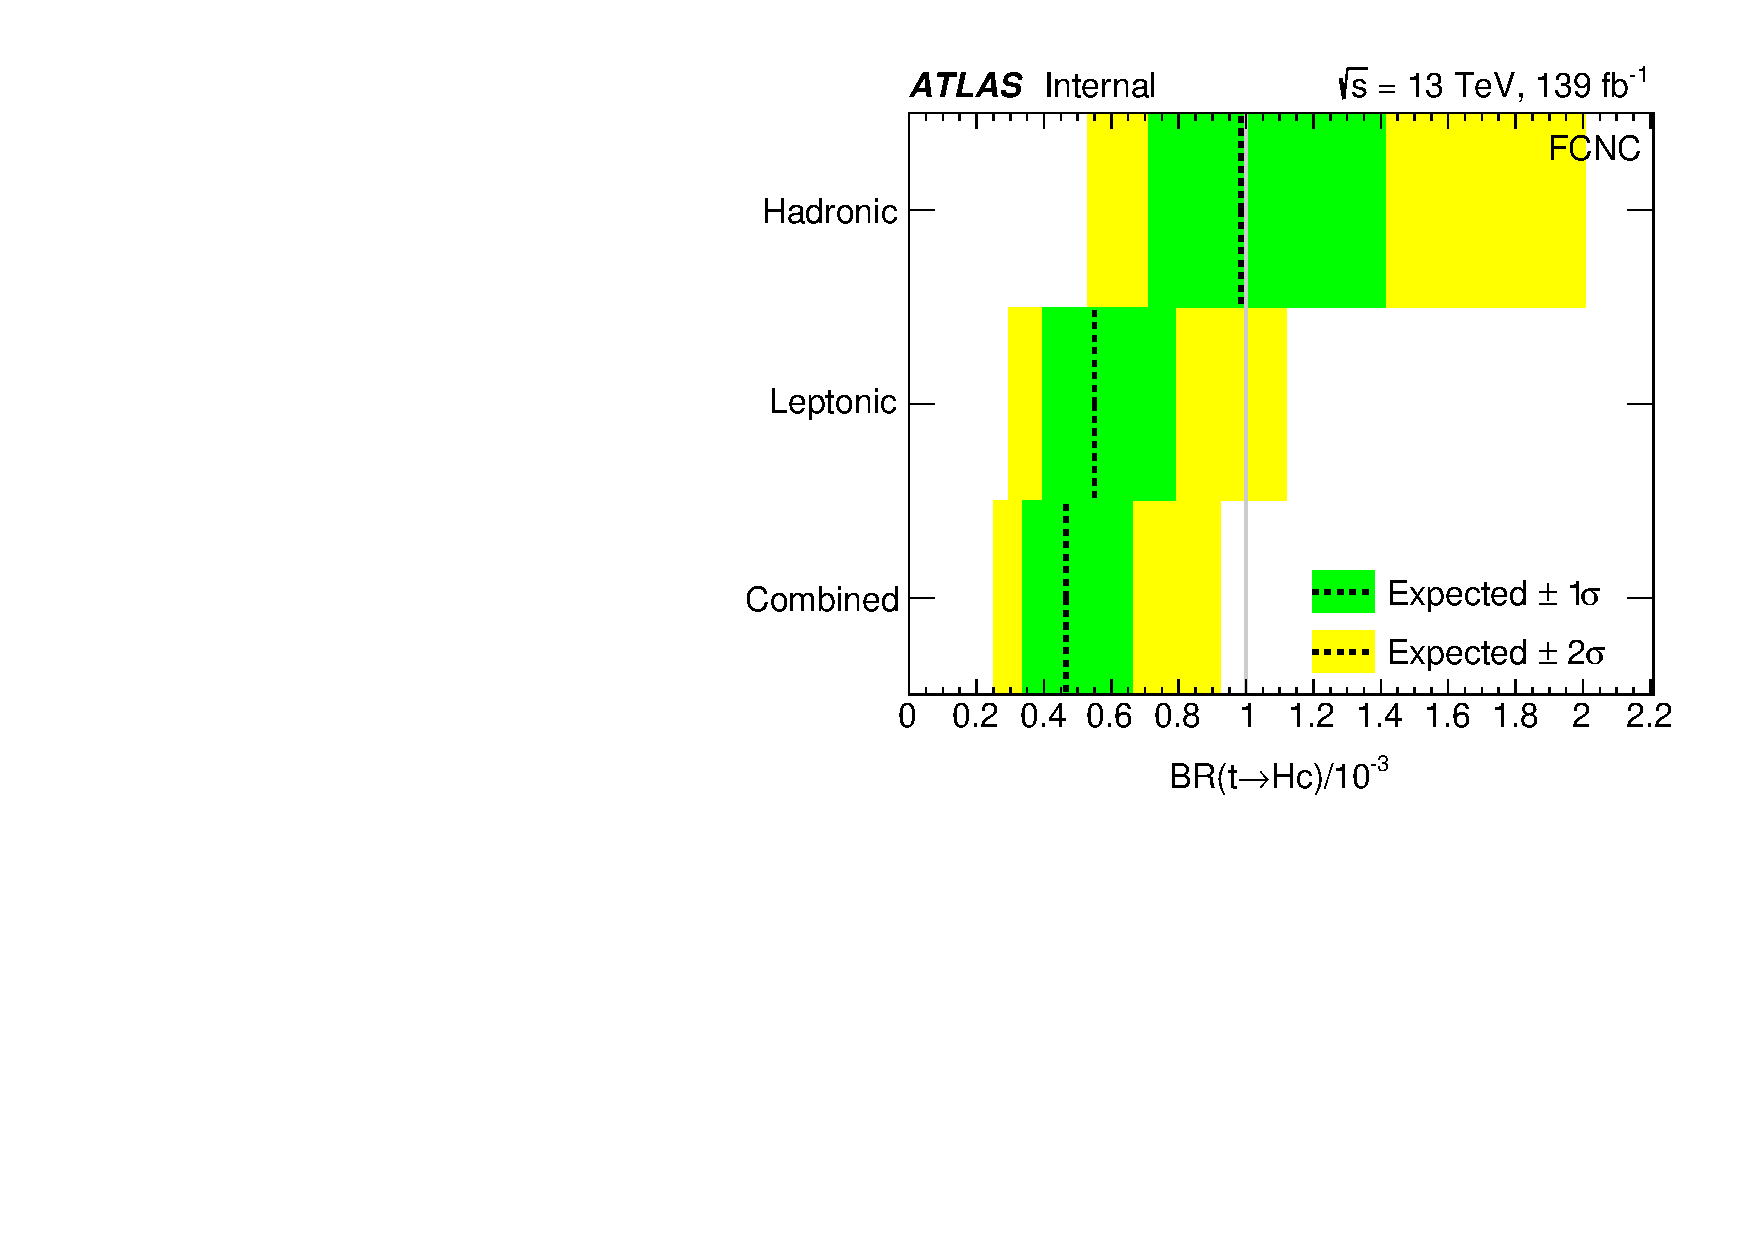
\includegraphics[width=0.7\textwidth]{\FCNCFigures/tcH_combined_Limit.pdf}
%\caption{\small {Summary of the best-fit $\BR(t\to Hc)$ for the individual channels as well as their combination,
%assuming $\BR(t\to Hu)=0$. (TBD: updated with best fit plots.)}}
%\label{fig:summary_printnum_hc} 
%\end{center}
%\end{figure*}
%%%%%%%%%%%%%%
%%%%%%%%%%%%%%
%\begin{figure*}[h!]
%\begin{center}
%\includegraphics[width=0.7\textwidth]{\FCNCFigures/tuH_combined_Limit.pdf}
%\caption{\small {Summary of the best-fit $\BR(t\to Hu)$ for the individual channels as well as their combination,
%assuming $\BR(t\to Hc)=0$. (TBD: updated with best fit plots.)}}
%\label{fig:summary_printnum_hu} 
%\end{center}
%\end{figure*}
%%%%%%%%%%%%%%

%The first set of combined results is obtained for each branching ratio separately, setting the other branching ratio to zero.
%The best-fit combined branching ratios are $\BR(t\to Hc)=[3.0^{+3.0}_{-2.7}\,(\mathrm{stat})^{+2.6}_{-2.1}\,(\mathrm{syst})] \times 10^{-4}$ and 
%$\BR(t\to Hu)=[4.2^{+3.2}_{-2.9}\,(\mathrm{stat})^{+2.6}_{-2.1}\,(\mathrm{syst})] \times 10^{-4}$.  
%%The difference between the central values of $\BR(t\to Hc)$ and $\BR(t\to Hu)$ originates from the ability of the $H \to b\bar{b}$ search to 
%%probe both decay modes separately.
%A comparison of the best-fit branching ratios for the individual searches and their combination is shown in Figure~\ref{fig:summary_printnum_hc} 
%for $\BR(t\to Hc)$ and Figure~\ref{fig:summary_printnum_hu} for $\BR(t\to Hu)$.
%The observed (expected) 95\% CL combined upper limits on the branching ratios are 
%$\BR(t\to Hc)<1.1 \times 10^{-3}\,(8.3 \times 10^{-4})$ and $\BR(t\to Hu)<1.2 \times 10^{-3}\,(8.3 \times 10^{-4})$.
A summary of the upper limits on the branching ratios obtained by the individual searches, as well as their combination, is given  
%%in Table~\ref{tab:limits_summary}, as is displayed in Figures~\ref{fig:limits_combo_1D_hc} and~\ref{fig:limits_combo_1D_hu}.
in Table~\ref{tab:limits_summary} and in Figures~\ref{fig:limits_combo_1D_hc}(a) and~\ref{fig:limits_combo_1D_hc}(b).

Upper limits on the branching ratios $\BR(t\to qH)$ ($q=u,c$) can be translated into upper limits on the dimension-6 (D6) operator Wilson coefficients appearing in the effective field theory Lagrangian for $tqH$ interaction~\cite{fcnc_production_theory}:
%
\begin{equation}
  \mathcal{L}_{EFT} = \frac{C^{i3}_{u\phi}}{\Lambda^{2}}(\phi^{\dagger}\phi)(\bar{q_{i}}t)\tilde{\phi} + \frac{C^{3i}_{u\phi}}{\Lambda^{2}}(\phi^{\dagger}\phi)(\bar{t_{i}}q)\tilde{\phi}
  \label{eq:eq01}
\end{equation}
%
where the subscript i= 1,2 represents the generation of the light quark fields ($q=u,c$).
The branching ratio $\BR(t\to qH)$ is estimated as the ratio of its partial width to the SM $t \to Wb$ partial width including next-to-leading-order QCD corrections and the coefficients can be extracted as $C_{q\phi} = \sqrt{1946.6~\BR(t\to qH)}$. The $C_{q\phi}$ coefficient corresponds to the sum in quadrature of the cofficients relative to the two possible chirality combinations of the quark fields,
$C_{q\phi} =\sqrt{(C^{i3}_{u\phi})^2 + (C^{3i}_{u\phi})^2}$~\cite{fcnc_production_theory}. The observed (expected) upper limits on the D6 Wilson coefficients from the combination of the searches are $C_{c\phi}<1.38\,(0.97)$ and $C_{u\phi}<1.18\,(0.83)$. 

%Upper limits on the branching ratios $\BR(t\to Hq)$ ($q=u,c$) can be translated into upper limits on the non-flavour-diagonal Yukawa couplings $\lamHq$ 
%appearing in the Lagrangian~\cite{Harnik:2012pb}:
%\begin{equation*}
%{\cal L}_\mathrm{FCNC} = -\lambda_{t_\mathrm{L} q_\mathrm{R}} \bar{t}_\mathrm{L} q_\mathrm{R} H - \lambda_{q_\mathrm{L} t_\mathrm{R}} \bar{q}_\mathrm{L} t_\mathrm{R} H  + \mathrm{h.c.}
%\end{equation*}
%The branching ratio $\BR(t\to Hq)$ is estimated as the ratio of its partial width~\cite{Zhang:2013xya} to the SM $t \to Wb$ partial width~\cite{Denner:1990ns}, 
%which is assumed to be dominant. Both predicted partial widths include next-to-leading-order QCD corrections.
%Using the expression derived in Ref.~\cite{Aad:2014dya}, the coupling $|\lamHq|$ can be extracted as $| \lamHq | = (1.92 \pm 0.02) \sqrt{\BR(t\to Hq)}$.
%The $\lamHq$ coupling corresponds to the sum in quadrature of the couplings relative to the two possible chirality combinations of the quark fields, 
%$\lamHq \equiv \sqrt{ |\lambda_{t_\mathrm{L} q_\mathrm{R}}|^2 +   |\lambda_{q_\mathrm{L} t_\mathrm{R}}|^2 }$~\cite{Harnik:2012pb}.
%The observed (expected) upper limits on the couplings from the combination of the searches are $|\lamHc|<0.064\,(0.055)$ and $|\lamHu|<0.066\,(0.055)$.

%%%%%%%%%%%%%%%
\begin{table}[t!]
\caption{\small{Summary of 95\% CL upper limits on $\BR(t \to cH)$ and $\BR(t \to uH)$, in each case neglecting the other decay mode. }}
\begin{center}
\begin{tabular}{lcc}
\toprule\toprule
 & \multicolumn{1}{c}{95\% CL upper limits} & \multicolumn{1}{c}{95\% CL upper limits}  \\
 & \multicolumn{1}{c}{on $\BR(t \to cH)$} & \multicolumn{1}{c}{on $\BR(t \to uH)$} \\
 &  Observed (Expected) & Observed (Expected)  \\
\midrule\midrule
hadronic  & $1.0 \times 10^{-5}$ ($9.8 \times 10^{-4}$) & $7.8 \times 10^{-4}$ ($7.8 \times 10^{-4}$) \\ 
leptonic  & $1.3 \times 10^{-5}$ ($5.9 \times 10^{-4}$) & $9.2 \times 10^{-4}$ ($4.2 \times 10^{-4}$) \\
\midrule
Combination  & $9.9 \times 10^{-4}$ ($5.0 \times 10^{-4}$) & $7.2 \times 10^{-4}$ ($3.6 \times 10^{-4}$) \\
\bottomrule\bottomrule
\end{tabular}
\label{tab:limits_summary}
\end{center}
\end{table}
%%%%%%%%%%%%%%%

%%%%%%%%%%%%%%
\begin{figure*}[h!]
\begin{center}
\begin{tabular}{@{}cc@{}}
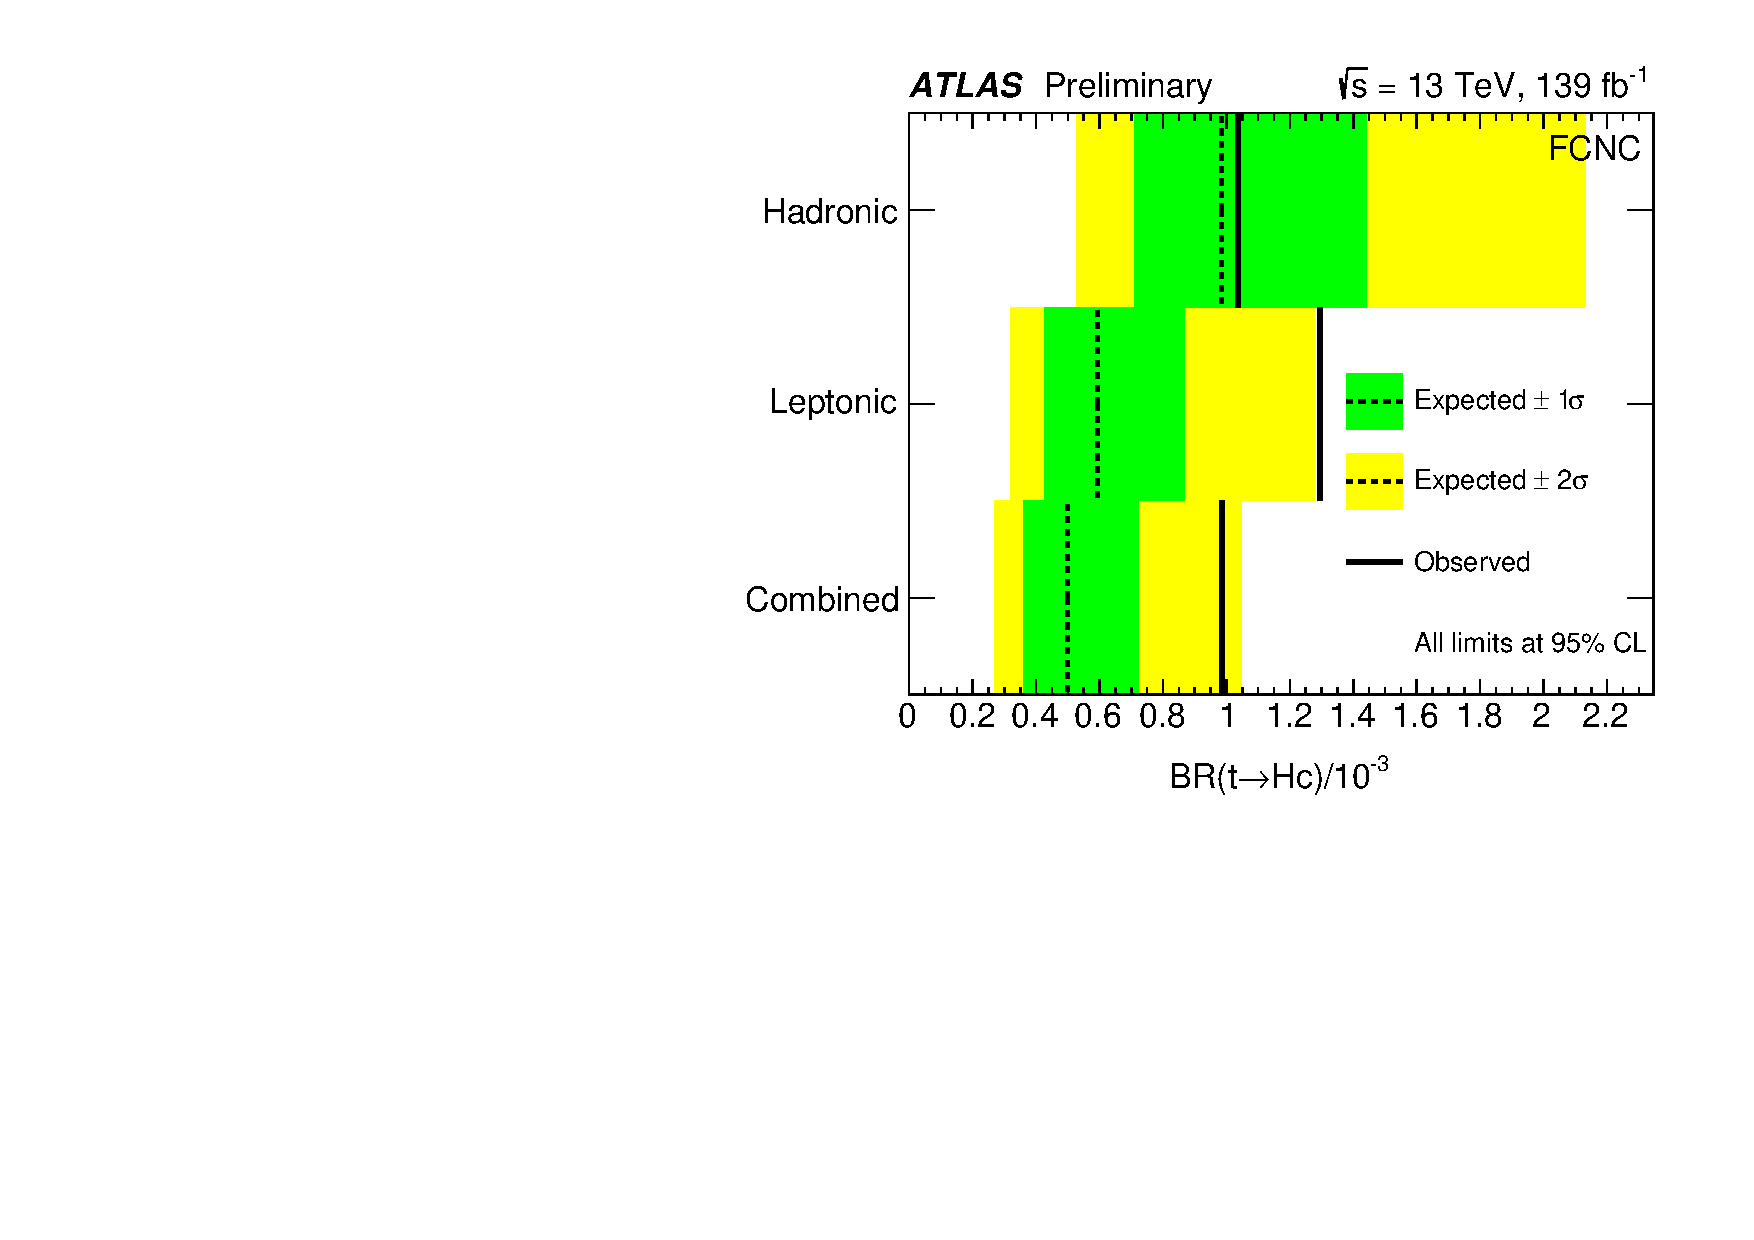
\includegraphics[width=0.49\textwidth]{figures/tcH_Limits.pdf}&
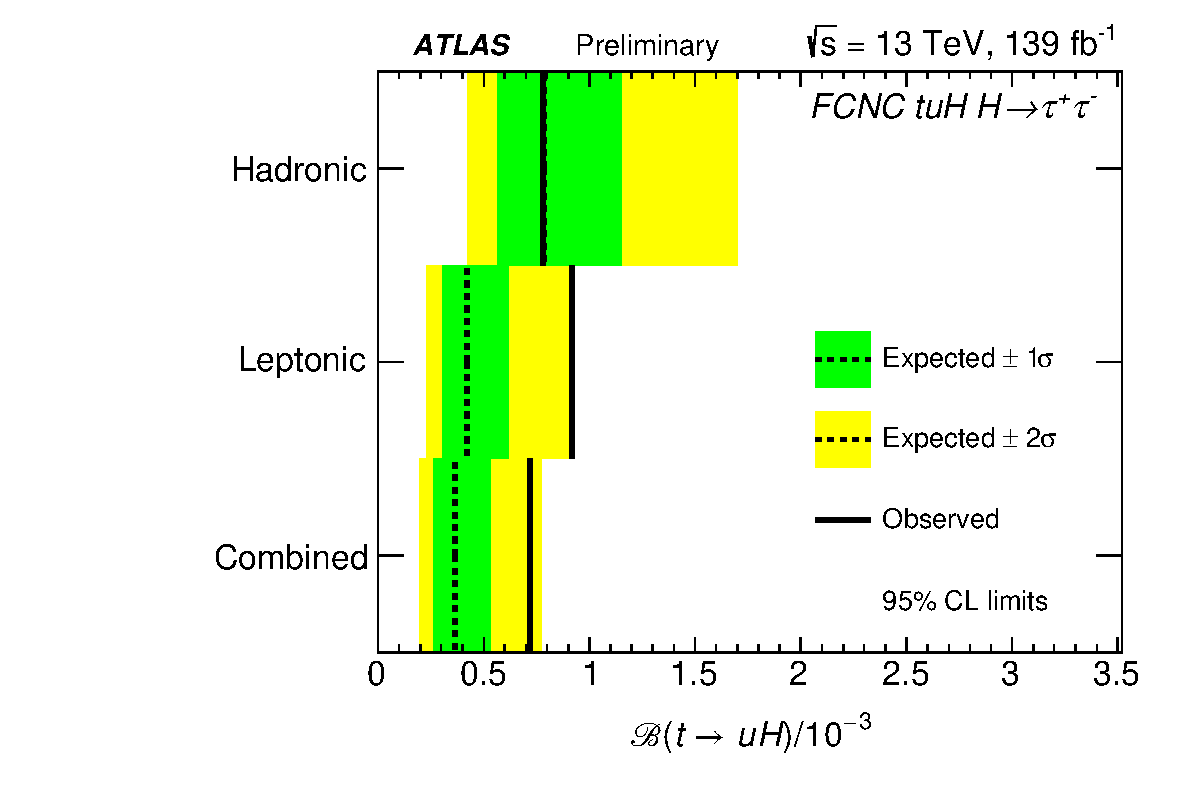
\includegraphics[width=0.49\textwidth]{figures/tuH_Limits.pdf}\\
(a) tcH & (b) tuH \\
\end{tabular}
\caption{\small {95\% CL upper limits on $\BR(t\to cH)$(a) for the individual searches as well as their
combination, assuming $\BR(t\to uH)=0$. 95\% CL upper limits on $\BR(t\to uH)$(b) for the individual searches as well as their
combination, assuming $\BR(t\to cH)=0$. The observed limits (solid lines) are compared with the 
expected (median) limits under the background-only hypothesis (dotted lines). The surrounding shaded bands correspond to the 68\% and 95\% CL intervals around the expected limits, 
denoted by $\pm 1\sigma$ and $\pm 2\sigma$, respectively.
}}
\label{fig:limits_combo_1D_hc} 
\end{center}
\end{figure*}
%%%%%%%%%%%%%%

%%%%%%%%%%%%%%%%%%
%%%%\begin{figure*}[h!]
%%%%\begin{center}
%%%%\includegraphics[width=0.7\textwidth]{figures/tuH_combined_Limit.pdf}
%%%%\caption{\small {95\% CL upper limits on $\BR(t\to Hu)$ for the individual searches as well as their
%%%%combination, assuming $\BR(t\to Hc)=0$. The observed limits (solid lines) are compared with the 
%%%%expected (median) limits under the background-only
%%%%hypothesis (dotted lines). The surrounding shaded bands correspond to the 68\% and 95\% CL intervals around the expected limits, 
%%%%denoted by $\pm 1\sigma$ and $\pm 2\sigma$, respectively.
%%%%}}
%%%%\label{fig:limits_combo_1D_hu} 
%%%%\end{center}
%%%%\end{figure*}

A similar set of results can be obtained by simultaneously varying both branching ratios in the likelihood function.
Figure~\ref{fig:limits_combo_2D}(a) shows the 95\% CL upper limits on the branching ratios in the $\BR(t\to uH)$ versus $\BR(t\to cH)$ plane. 
%The small differences between the limiting values (on the $x$- and $y$-axes) of the branching ratio limits obtained in the two-dimensional scan and 
%those reported in Table~\ref{tab:limits_summary}, result from slightly different choices in the $\HML$ search  
%regarding the final discriminant, which in the two-dimensional case should be common to both signals, and its binning.
%\textbf{Add comment of what discriminant is used in this case and the caveat regarding the corresponding 1D limit.}
The corresponding upper limits on the D6 Wilson coefficients couplings in the $C_{u\phi}$ versus $C_{c\phi}$ plane are shown in Figure~\ref{fig:limits_combo_2D}(b).

\begin{figure*}[t!]
\begin{center}
\subfloat[]{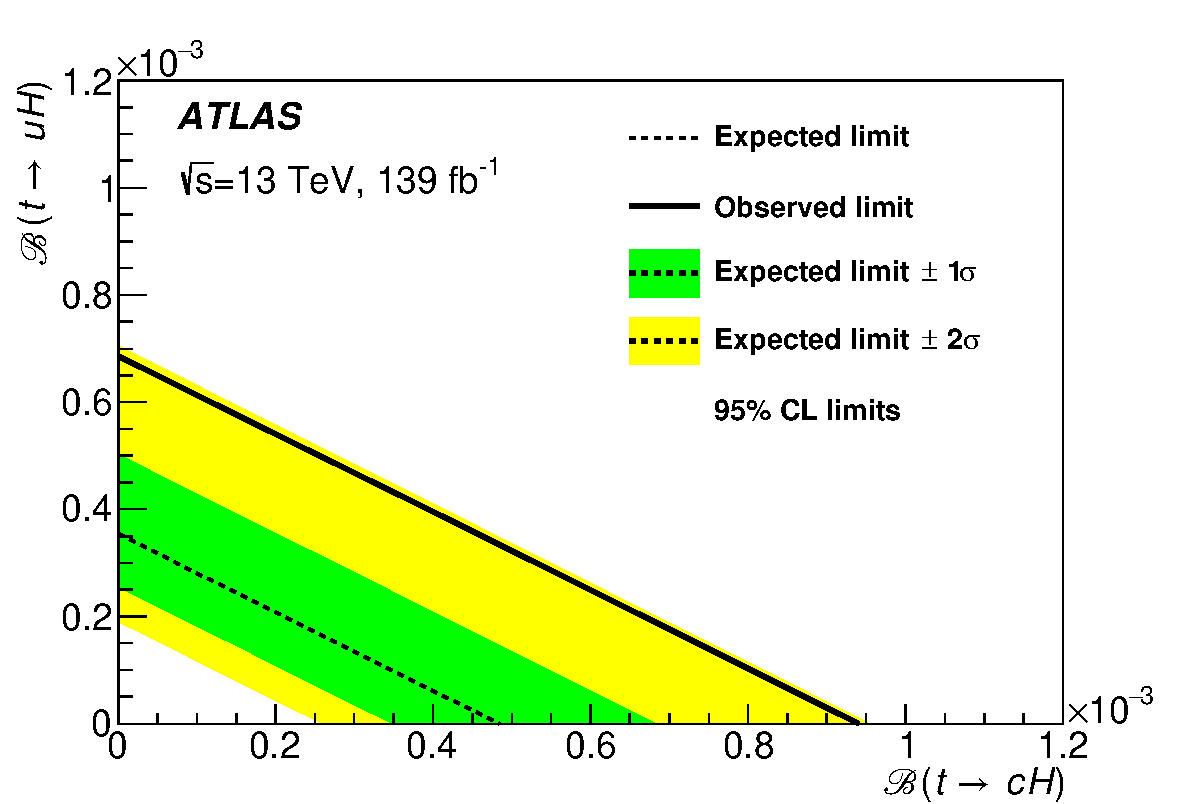
\includegraphics[width=0.49\textwidth]{figures/2DLimits.pdf}}
\subfloat[]{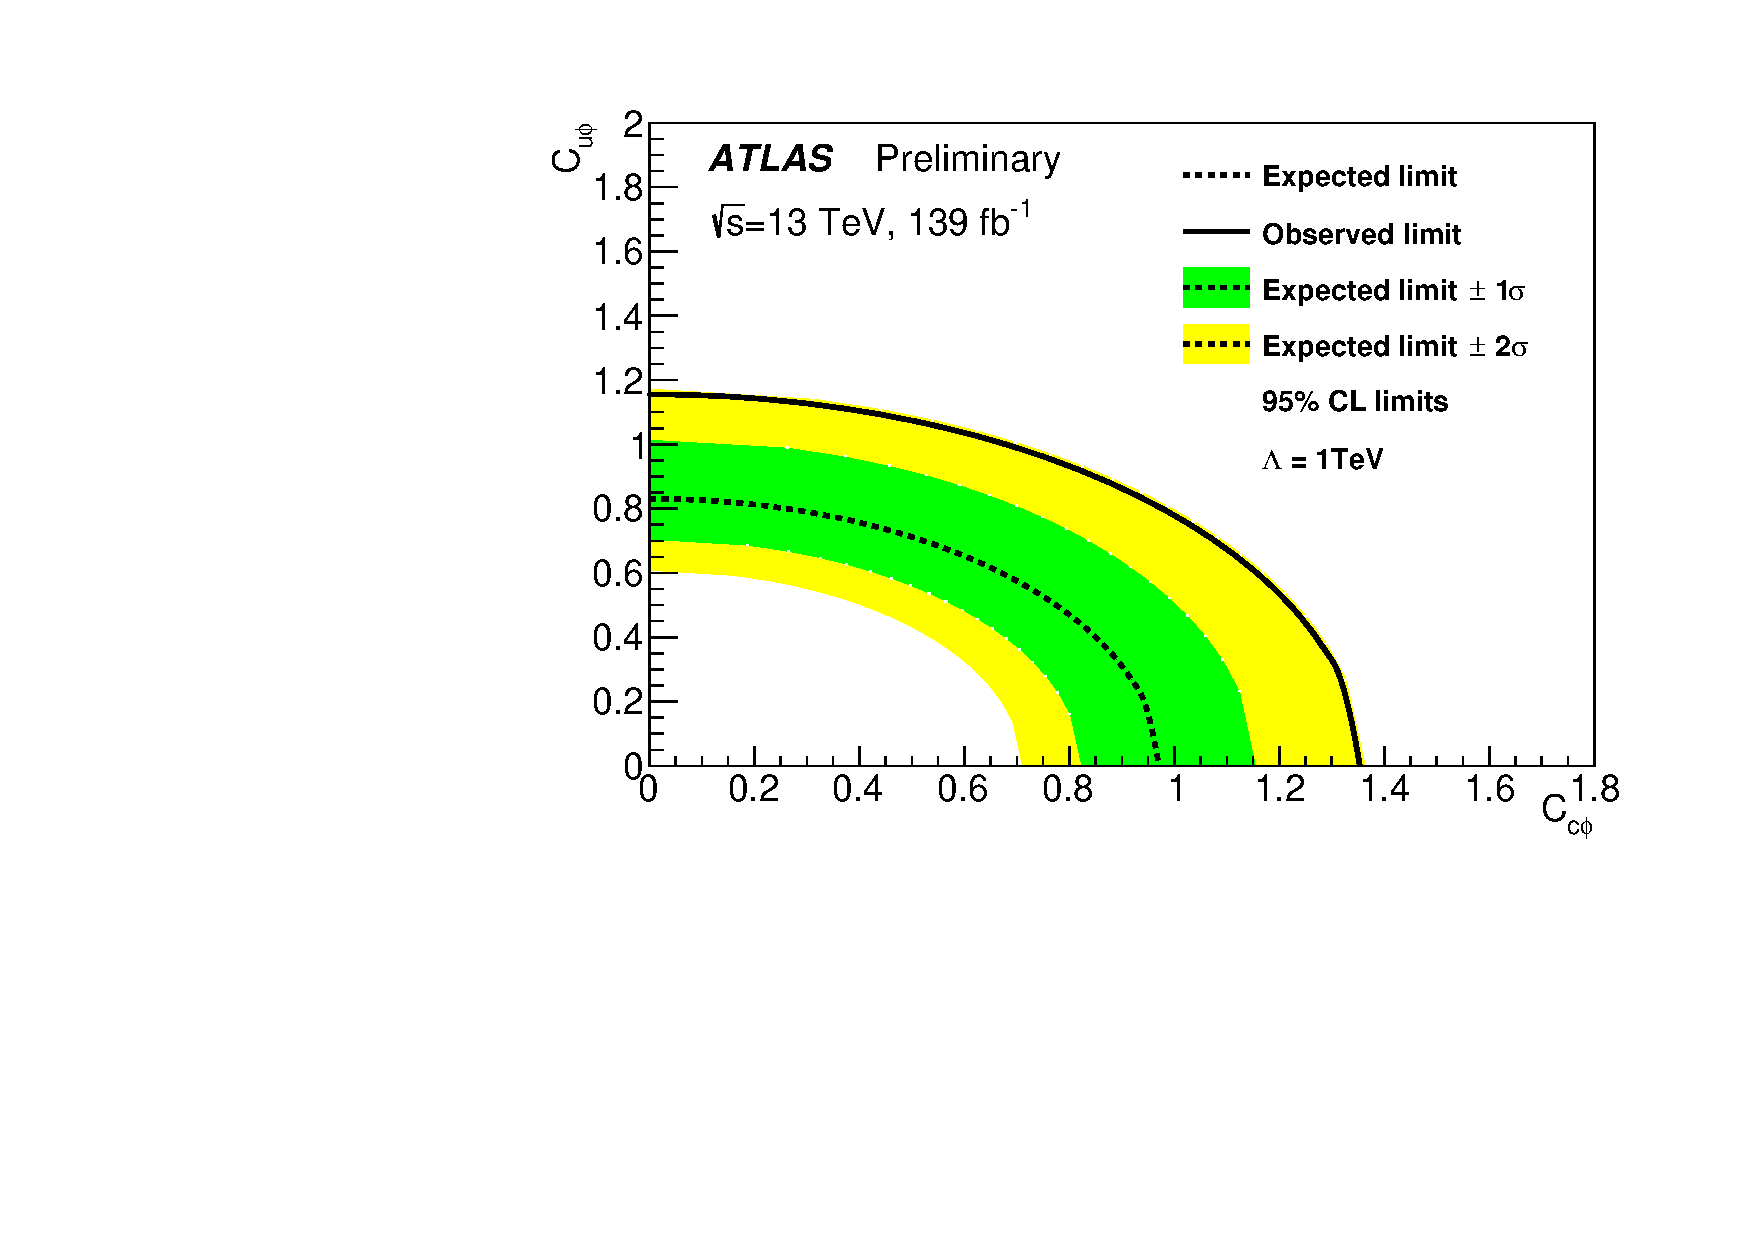
\includegraphics[width=0.49\textwidth]{figures/Wilson_coefficient_smooth.pdf}}
\caption{\small {95\% CL upper limits (a) on the plane of $\BR(t\to uH)$ versus $\BR(t\to cH)$ and (b) on the plane 
of $C_{c\phi}$ versus $C_{u\phi}$ for the combination of the searches. The observed limits (solid lines) are compared with the expected (median) limits under the background-only hypothesis (dotted lines). The surrounding shaded bands correspond to the 68\% and 95\% CL intervals around the expected limits, 
denoted by $\pm 1\sigma$ and $\pm 2\sigma$, respectively.}}
%%=======
%%of $C_{u\phi}$ versus $C_{c\phi}$ for the combination of the searches. The observed limits (solid lines) are compared with the expected (median) limits under the background-only hypothesis (dotted %%lines). The surrounding shaded bands correspond to the 68\% and 95\% CL intervals around the expected limits, 
%%denoted by $\pm 1\sigma$ and $\pm 2\sigma$, respectively. ({\color{red} plot (b) needs to be updated}) }}
%%>>>>>>> e84999e0023e50e93b4b7507152380195248366c
\label{fig:limits_combo_2D} 
\end{center}
\end{figure*}
%%%%%%%%%%%%%%


